\documentclass{article}

%\begin{figure}[h]
%\begin{center}
%\caption{\label{1} titre}
%\includegraphics[scale=0.5]{{nom_photo}.png}
%\captionsetup{labelformat=empty}
%\caption{ sources : nom_source}
%\end{center}
%\end{figure}

% \begin{center}
% \begin{tabular}{|c|c|}
			% \hline
			% a & a \\
			
			% a & a  \\
			% \hline
			% a & a \\
			
			% a & a  \\
			% \hline
			% a & a \\
			
			% a & a  \\
			% \hline
% \end{tabular}
% \end{center}

%[ForwardSearch("%bm.pdf","%Wc",%l,0,0,1)]


\usepackage[utf8]{inputenc}
\usepackage[T1]{fontenc}
\usepackage[french]{babel}
\usepackage{amsmath}
\usepackage{amssymb}
\usepackage{graphicx}
\usepackage{caption}
\usepackage{subcaption}
\usepackage{fancyhdr}
\usepackage{gensymb}
\usepackage{array}
\usepackage{caption}
%\usepackage[left=2cm,right=2cm,top=2cm,bottom=2cm]{geometry}
%\usepackage[left=2cm,right=2cm,top=2cm,bottom=2cm]{geometry}
%\newgeometry{top=1in,bottom=1in,right=0.5in,left=1.5in}

\usepackage{listings}
\usepackage{color}

\definecolor{dkgreen}{rgb}{0,0.6,0}
\definecolor{gray}{rgb}{0.5,0.5,0.5}
\definecolor{mauve}{rgb}{0.58,0,0.82}

\lstset{frame=tb,
  language=Python,
  aboveskip=3mm,
  belowskip=3mm,
  showstringspaces=false,
  columns=flexible,
  basicstyle={\small\ttfamily},
  numbers=none,
  numberstyle=\tiny\color{gray},
  keywordstyle=\color{blue},
  commentstyle=\color{dkgreen},
  stringstyle=\color{mauve},
  breaklines=true,
  breakatwhitespace=true,
  tabsize=3
}

\renewcommand{\thesection}{\Roman{section}}
\renewcommand{\thesubsection}{\arabic{subsection}}


\newcommand{\deriv}[2]{\frac{\partial #1}{\partial #2}}
\DeclareMathOperator{\Tr}{Tr}
\title{Machine learning pour la classification de phases de sommeil}
\author{Alexandre Herbert et Baptiste Turpin}
\date{}
\begin{document}

\maketitle

\newpage

\setcounter{tocdepth}{2}
\renewcommand{\contentsname}{Sommaire}
\tableofcontents

\newpage

\section{Contexte}

Le sommeil tient une place majeure dans notre santé et notre bien-être. Il se décompose en une succession de phases répétées par cycle :
\\
\begin{itemize}
\item Phase 0 : endormissement (individu réveillé)
\item Phase 1 : sommeil léger
\item Phases 2 et 3 : sommeil profond
\item Phase 4 : sommeil paradoxal ou REM (Rapid Eye Movement)
\end{itemize}
\vspace{0.5cm}

Le travail de DREEM repose sur la mise en place de solutions permettant de diagnostiquer les problèmes de sommeil. Il s'agit d'identifier lors d'une session de sommeil l'enchainement des différentes phases pour comprendre l'origine du trouble. A cette fin, DREEM a lancé sur le marché un bandeau permettant de récupérer 3 catégories de signaux pendant le sommeil de l'individu :
\\
\begin{itemize}
\item L'activité éléctrique du cerveau (par 7 électroencéphalographie)
\item L'accélération (par 3 accéléromètrie)
\item L'absorption de la lumière infrarouge par l'hémoglobine, caractéristique de la teneur en oxygène du sang (par 1 oxymétrie colorimétrique)
\end{itemize}
\vspace{0.5cm}

L'objectif est de prédire la phase du sommeil à partir de ces 11 signaux relevés. A cette fin, DREEM travaille sur un modèle d'apprentissage supervisé pour la classification en 5 phases de sommeil. Des spécialistes du sommeil ont donc été sollicité pour étiqueter un ensemble d'échantillons, chaque échantillon étant constitué des 11 signaux capturés sur une période de 30".
\\
L'objectif du présent projet est :
\\
\begin{itemize}
\item De sélectionner un modèle de Machine Learning et des hyperparamètres efficaces pour le problème de classification proposé
\item D'identifier des features pertinents pour chacun des signaux permettant de discriminer les phases du sommeil
\item D'appliquer la technique d'apprentissage par validation croisée et un prétraitement des données adapté au problème
\end{itemize}
\vspace{0.5cm}

Nous reviendrons dans ce qui suit sur les différents choix que nous avons opérés : modèle, prétraitement, extraction de features, entrainement. Nous présenterons ensuite de manière critique les résultats obtenus, avant d'envisager des perspectives d'amélioration.

\section{Choix d'implémentation}
\subsection{Choix du modèle}

Dans un tout premier temps, nous avons utilisé un apprentissage non-supervisé de type k-means. Cette méthode, très peu performante, visait juste à évaluer la qualité des features extraits, pour savoir s'ls permettaient de discriminer efficacement les phases du sommeil. Aucune performance probante n'a pu être tirée de cette analyse.
\\

L'analyse de l'existant nous a ensuite rapidement orienté vers les modèles évalués comme étant les plus performants pour ce problème : le Random Forest ou le simple decision tree.
\\

Nous nous sommes finalement tournés vers le Random Forest, afin d'obtenir une classification plus fine qu'un simple decision tree, et puisque nous ne cherchons pas ici à déterminer un sens "physique" pour les noeuds.
\\

Nous avons cherché à optimiser les hyperparamètres suivants (attributs de la classe sklearn.ensemble.RandomForestClassifier) :
\\

\begin{itemize}
\item Le nombre d'arbres de la forêt (n\_estimators)
\item Le critère de qualité d'une division (criterion)
\item La profondeur maximale (max\_depth)
\item Le nombre minimal d'échantillons pour une division (min\_samples\_split)
\item Le nombre minimal d'échantillons par feuille (min\_samples\_leaf)
\item Le taux minimal de réduction du critère de qualité autorisant une division (min\_impurity\_decrease)
\end{itemize}
\vspace{0.5cm}

TABLEAU MONTRANT UN CROISEMENT DES PARAMETRES POUR OPTIMISATION ?
\\

Finalement, les valeurs suivantes ont été choisies pour ces hyperparamètres :
\\

\begin{center}
 \begin{tabular}{|c|c|}
			 \hline
			 \textbf{Hyperparamètre} & \textbf{Valeur} \\
			 \hline
			 n\_estimators & ?  \\
			 \hline
			 criterion & ? \\
			 \hline
			 max\_depth & ?  \\
			 \hline
			 min\_samples\_split & ? \\
			 \hline
			 min\_samples\_leaf & ?  \\
			 \hline
			 min\_impurity\_decrease & ?  \\
			 \hline
 \end{tabular}
\end{center}

\subsection{Sélection des méthodes de validation algorithmique}

L'apprentissage est réalisé par validation croisée. Le découpage du dataset d'entrainement est réalisé avec la classe 
\newline sklearn.model\_selection.StratifiedKFold. Le nombre de folds (n\_folds) a été fixé à 5. Le dataset est mélangé alétaoirement (shuffle = True).

Nous calculons à partir de cet apprentissage le F1-score ainsi que la matrice de confusion obtenus par la validation.

\section{Selection de features}

Nous avons dans un premier temps affiché les signaux temporels du dataset d'entrainement afin d'établir des caractéristiques des différentes phases de sommeil.
\\

\begin{figure}[h]
\begin{center}
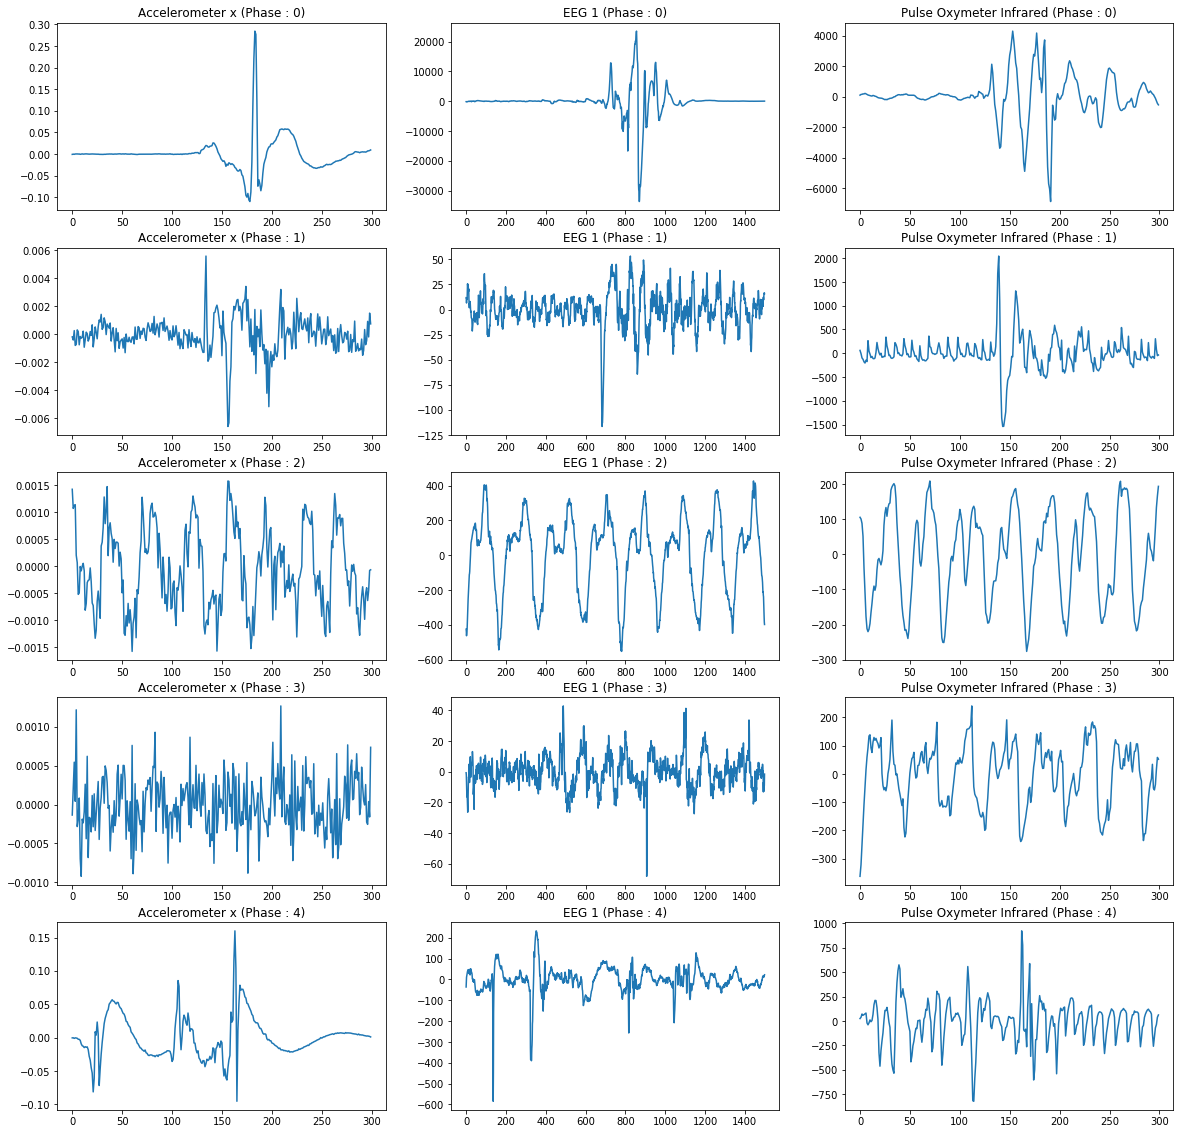
\includegraphics[scale=0.3]{{images/temp_signals}.png}
\caption{Signaux temporels pour différentes phases}
\end{center}
\end{figure}

\clearpage

Nous pouvons faire les premières observations suivantes :
\\

\begin{itemize}
\item Les signaux de la phase 0 sont d'amplitude très élevée, mais avec de faibles fluctuations, et sans motif répété.
\item L'accéléromètre de la phase 4 ne présente que peu de fluctuation, et aucun motif répété.
\end{itemize}
\vspace{0.5cm}

Plus généralement, on constate que :
\\

\begin{itemize}
\item Les signaux se composent de motifs répétés pour les phases 1, 2 et 3.
\item La forme des motifs, leur amplitude et leur fréquence d'apparition semble varier en fonction de la phase
\end{itemize}
\vspace{0.5cm}

Cela nous amène à considérer en supplément les caractéristiques fréquentielles des signaux. Nous avons calculé la valeur absolue de la transformée de Fourier des signaux temporels (figure 2).
\\


\begin{figure}[h]
\begin{center}
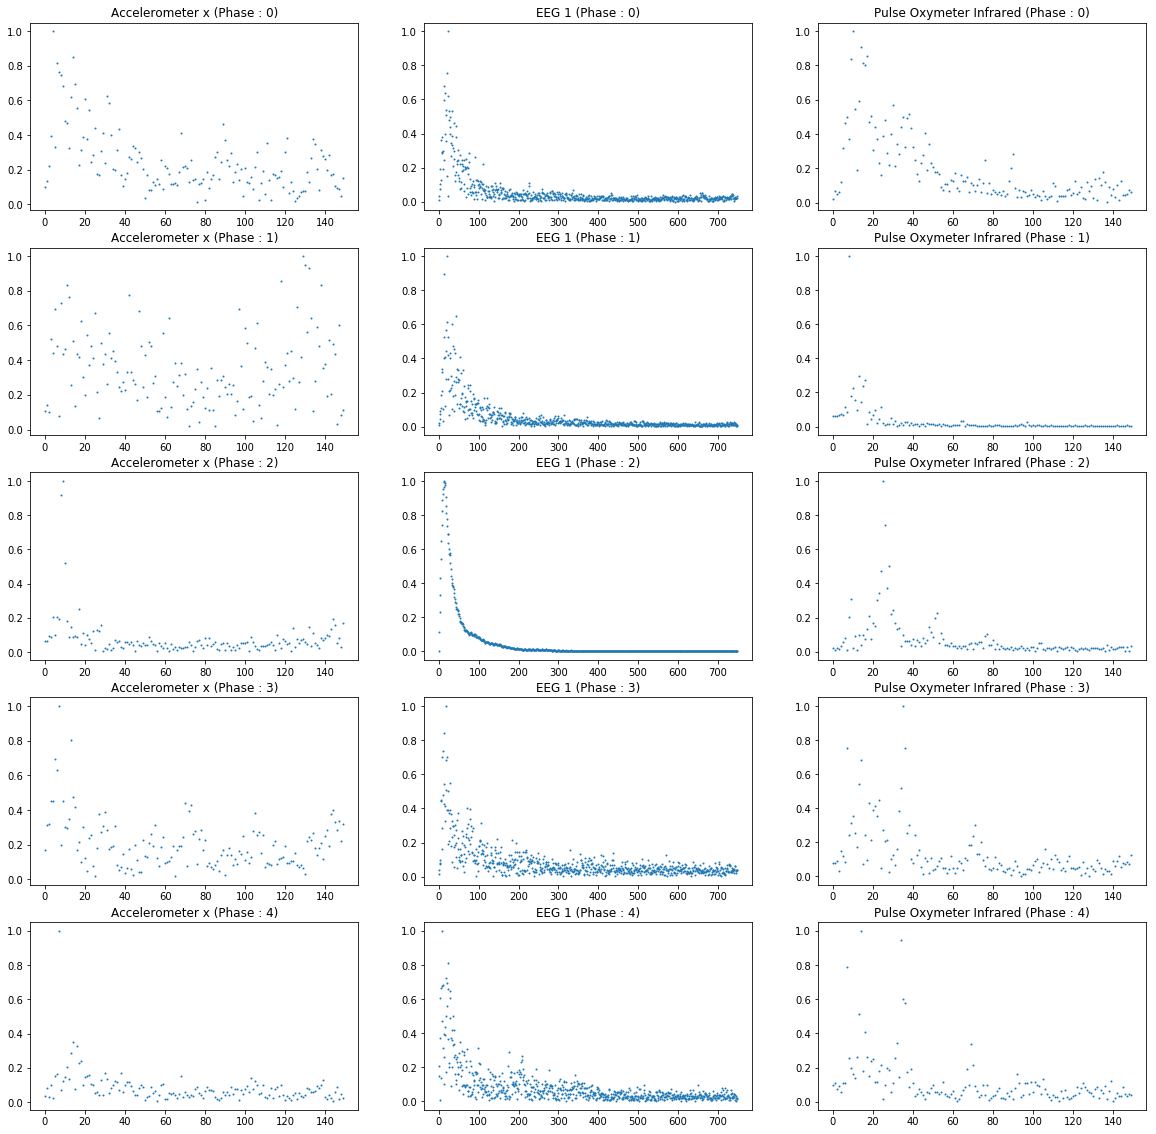
\includegraphics[scale=0.3]{{images/freq_signals}.png}
\caption{FFT des signaux pour différentes phases}
\end{center}
\end{figure}


On constate sur la comparaison des FFT que l'amplitude maximale observée varie beaucoup en fonction de la phase. En outre, en ne considérant que la forme de la FFT et la distribution des points dasn la fenêtre d'affichage, on tire les observations suivantes :
\\

\begin{itemize}
\item EEGs : la FFT est plus ou moins bien dessinée en fonction de la phase : pour une plage de fréquences réduite donnée, il semblerait que la variance en amplitudes des différents points soit plus ou moins forte. Dans le cas ci-dessus, la phase 2 est bien dessinée, tandis que les phases 3 et 4 présente un nuage de points étendu.
\item Accéléromètres : des points isolés en haut à droite de la fenêtre d'affichage peuvent être observés sur les phases 0, 1 et 3.
\item Oxymétrie colorimétrique : on distingue plusieurs pics, qui sont plus ou moins espacés et d'amplitudes plus ou moins équilibrées en fonction des phases.
\end{itemize}
\vspace{0.5cm}

De toutes ces observations, nous avons décidé d'extraire les features suivants. Dans la description, "signal" est la liste des ordonnées du signal : ordonnées temporelles (resp fréquentielles), suivant que la méthode est appliquée au signal temporel (resp à la FFT) ) :
\\

\textbf{distanceMinMax} \\
La liste signal est partitionnée en n intervalles disjoints : $signal = \bigcup\limits_{i=1}^n signal_i$. \\
Puis distanceMinMax = $\sum\limits_{i=1}^n max(signal_i) - min(signal_i)$.  \\\\

\textbf{maxAmp} \\
maxAmp = $max(signal)$ \\\\

\textbf{freqMinLimitAmp} \\
Soit une amplitude A donnée. \\
freqMinLimitAmp = $min(f_t)$ tq $\forall f > f_t, signal(f)< A$\\\\

\textbf{nbPikes} \\
Soit une amplitude A et une largeur d'intervalle W données.\\
Un intervalle de largeur W signal$_{ext}$ extrait de signal est un unique pic ssi $min(signal_{ext})>A$.  \\
nbPikes est le nombre de pics distincts de signal. \\

\textbf{indexMaxAmp} \\
Soit une largeur d'intervalle W. \\
indexMaxAmp = $\underset{len(signal_{ext})=W}{\underset{signal_{ext}\subset signal}{\text{argmax}}} mean(signal_{ext})$

\textbf{meanDiffNeighb} \\
Soit une largeur d'intervalle W. \\


\textbf{stdDeviationNb} \\

\textbf{upperRight} \\
Soit une amplitude A et une abscisse x. upperRight = $\sum\limits_{a>x}(\mathbf{1}(signal(a)>A))$.

\textbf{mean} \\
mean = mean(signal)

\textbf{meanOfAbs} \\
meanOfAbs = mean(abs(signal))

\textbf{maxOfAbs} \\
maxOfAbs = max(abs(signal))

\textbf{minOfAbs} \\
minOfAbs = min(abs(signal))

\section{Pré-traitement des données}

Nous avons dans un premier temps pu constater que le dataset d'entrainement est déséquilibré :
\\


\begin{figure}[h]
\begin{center}
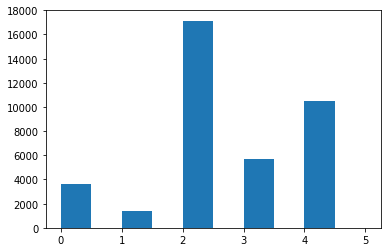
\includegraphics[scale=0.5]{{images/hist}.png}
\caption{Distribution du dataset d'entrainement entre les classes}
\end{center}
\end{figure}


Pour cette raison, nous avons appliqué deux méthodes :\\

\begin{itemize}
\item Réaliser la validation croisée sur un dataset équilibré entre les classes : tous les échantillons de la classe 1 (la moins représentée avec 1353 échantillons) sont conservés ; les échantillons des autres classes sont tirés aléatoirement. On passe ainsi d'un dataset de 38289 échantillons à un nouveau dataset équilibré de 6765 échantillons. 
\item Réaliser la validation croisée sur l'ensemble du dataset, et appliquer des poids aux classes pour pénaliser les mauvais classements associés aux classes les moins représentées.
\end{itemize}
\vspace{0.5cm}

Par ailleurs, la valeur absolue de la FFT d'un signal est symétrique. Nous pouvons donc nous contenter de la première moitié de cette FFT. \\

Enfin, pour certains features, on désire extraire de l'information dans la forme du signal ou de la FFT. Dans ce cas précis, les amplitudes sont normalisées dans la fourchette [0,1].\\

\section{Optimisation des hyperparamètres des features}

Certains features listés plus tôt présentent des hyperparamètres : amplitude, largeur d'intervalle, abscisse. Nous avons décidé d'optimiser les valeurs de ces hyperparamètres séparément. Nous avons donc réalisé des apprentissages par validation croisée pour toutes les matrices de design élémentaires. Chaque matrice de design élémentaire est constituée d'un seul feature, appliqué à une seule catégorie de signal (EEG, accéléromètre ou oxymétrie colorimétrique), soit sur le signal temporel ou sur la FFT.\\

Le but de cette optimisation est double :\\
\begin{itemize}
\item Identifier parmi les familles (feature, catégorie de signal, temporel/fréquentiel) celles qui apportent les meilleurs résultats (cad dont le score-F1 atteint est le plus élevé)
\item Trouver les valeurs des hyperparamètres les plus pertinentes pour chaque famille (feature, catégorie de signal, temporel/fréquentiel)
\end{itemize}
\vspace{0.5cm}

Voici ci-dessous un extrait de l'analyse opérée :\\

EXTRAIT DU TABLEAU
\\

A l'issue de cette analyse, nous avons conservé les features suivants pour notre modèle :\\

TABLEAU
\\

La matrice de design finale, obtenue par concaténation des matrices élémentaires, contient donc XXX colonnes.\\



\section{Résultats}

\section{ Critiques et perspectives}

Comme expliqué précédemment, nous avons optimisé les hyperparamètres des features en validation croisée. En travaillant ainsi, nous savions qu'il y avait un risque d'overfitter les set de validation. Ce phénomène s'est révélé être bien plus important que nous ne le craignions, et le F1-score obtenu sur le dataset de test était nettement plus faible que celui obtenu en validation croisée.



\begin{lstlisting}
X_test_fft = h5py.File('data/X_test_fft.h5')

def buildAndSaveMatrix(h5file_freq, methodOne, param, list_bool_extract_signal, name_save):
    rep = extractFeatureAll(h5file_freq , methodOne , param , list_bool_extract_signal)
    temp_var_file = open("design_matrix/elem/" + name_save + '.txt','wb')
    pickle.dump(rep , temp_var_file)
    temp_var_file.close()
		len(bidule)
\end{lstlisting}


\end{document}
